\documentclass[pdflatex,sn-mathphys-num]{sn-jnl}

\usepackage{graphicx}
\usepackage{multirow}
\usepackage{amsmath,amssymb,amsfonts}
\usepackage{amsthm}
\usepackage{mathrsfs}
\usepackage[title]{appendix}
\usepackage{xcolor}
\usepackage{textcomp}
\usepackage{manyfoot}
\usepackage{booktabs}
\usepackage{algorithm}
\usepackage{algorithmicx}
\usepackage{algpseudocode}
\usepackage{listings}

\raggedbottom

\begin{document}

\title[Random Forest global para el pronóstico de ventas minoristas]{Pronóstico mensual de ventas minoristas por categoría y región con un Random Forest global sobre un índice libre de escala: evaluación con pruebas de capacidad predictiva en Sample Superstore}

\author[1]{\fnm{Alex} \sur{Teran}}

\author[1]{\fnm{David} \sur{Estrada}}

\affil[1]{\orgname{Universidad del Norte}, \orgaddress{\city{Barranquilla}, \country{Colombia}}}

\abstract{La planificación comercial de una cadena minorista requiere pronósticos mensuales de ventas por categoría y región, pero a ese nivel las series son cortas, ruidosas y de escalas distintas. Este trabajo formula el problema como una regresión supervisada sobre el conjunto público Sample Superstore (9{,}994 líneas de pedido, 2014--2017), agregado en un panel de 12 series y 48 meses, y propone un Random Forest global que predice un índice de ventas libre de escala (ventas del mes divididas por el promedio de los doce meses previos) y se aplica de forma recursiva a horizontes de doce meses. El modelo se comparó con un pronóstico ingenuo estacional y con siete regresores (Ridge, Lasso, regresión bayesiana, KNN, árbol de decisión, XGBoost y SVR) bajo la misma partición temporal, el mismo preprocesamiento y búsqueda en rejilla con validación cruzada temporal. En 2017, reservado como prueba, el modelo propuesto obtuvo un MAE de 2{,}634 $\pm$ 834 USD por serie y mes, 9.5\% menor que el del ingenuo estacional, y desvió el total anual en $+0.7$\% (frente a $-16.9$\%). Sin embargo, las pruebas de Diebold--Mariano, Giacomini--White y bayesiana con región de equivalencia práctica, corregidas por Holm, no aportan evidencia de diferencia significativa frente a ningún modelo de referencia; SVR logró un MAE menor a costa de subestimar el total en 13.8\%, y el Random Forest fue el modelo más costoso (0.36 s de ajuste). La ablación sugiere que el índice no reduce el error por serie, pero sí corrige el sesgo del total.}

\keywords{Pronóstico de ventas minoristas, Regresión supervisada, Random Forest global, Índice libre de escala, Error absoluto medio, Prueba de Diebold--Mariano}

\maketitle

\section{Introducción}\label{sec:intro}

Pronosticar las ventas es un insumo directo de la planificación minorista: de la cifra esperada dependen las metas de cada región, las compras de inventario de cada categoría y el presupuesto de ingresos del año siguiente \cite{fildes2022}. Esas decisiones no se toman sobre el total de la empresa sino sobre combinaciones de producto y territorio, y a ese nivel de desagregación las series son más cortas, más ruidosas y de tamaños muy distintos entre sí, lo que dificulta tanto el ajuste de un modelo como la comparación honesta entre varios \cite{fildes2022,hyndman2021}.

La práctica habitual en empresas pequeñas y medianas es proyectar ``lo mismo que el mismo mes del año anterior''. Este pronóstico ingenuo estacional captura la estacionalidad sin estimar ningún parámetro y es la referencia mínima que cualquier método debe superar \cite{hyndman2021}, pero arrastra el nivel de hace doce meses: cuando la empresa crece, subestima de forma sistemática. Los modelos de aprendizaje automático ofrecen una alternativa. Las competencias recientes de pronóstico, en particular M5 con ventas minoristas jerárquicas, mostraron que los ensambles de árboles entrenados sobre muchas series a la vez dominan a los métodos que ajustan cada serie por separado \cite{makridakis2022}, y la teoría de los modelos globales explica por qué: compartir parámetros entre series aumenta el tamaño efectivo de la muestra sin sacrificar, en principio, capacidad de representación \cite{monteromanso2021}.

Tres limitaciones impiden trasladar directamente esos resultados a un panel pequeño. Primera, un modelo global necesita que las series sean comparables; las soluciones más exitosas normalizan cada serie por su nivel antes de modelarla \cite{salinas2020,smyl2020}, mientras que la aplicación directa de regresores estándar sobre ventas en dólares mezcla series grandes y pequeñas. Segunda, los ensambles de árboles (Random Forest \cite{breiman2001}, XGBoost \cite{chen2016}) no extrapolan fuera del rango observado en entrenamiento, de modo que una tendencia creciente los sesga hacia abajo. Tercera, con pocos meses de prueba las diferencias entre modelos suelen ser menores que su variabilidad, y una tabla de errores promedio sin pruebas de capacidad predictiva \cite{diebold1995,giacomini2006} ni corrección por comparaciones múltiples \cite{holm1979} puede atribuir al modelo lo que es azar de la partición \cite{cerqueira2020}.

Este trabajo aborda el problema sobre el conjunto público Sample Superstore \cite{superstore}, que registra las ventas de una cadena minorista de Estados Unidos entre 2014 y 2017 en tres categorías de producto y cuatro regiones. Las contribuciones son tres. (i) Se formula el pronóstico mensual por categoría y región como una regresión supervisada sobre un \emph{índice de ventas libre de escala}, las ventas del mes divididas por el promedio de los doce meses anteriores de la misma serie, con rezagos expresados en la misma unidad y una codificación cíclica del mes; el índice hace comparables las series y vuelve estacionario el nivel que los árboles no pueden extrapolar. (ii) Se propone un Random Forest global entrenado sobre las doce series agrupadas y aplicado de forma recursiva para proyectar doce meses, y se compara con el ingenuo estacional y con siete regresores (Ridge \cite{hoerl1970}, Lasso \cite{tibshirani1996}, regresión bayesiana \cite{mackay1992}, KNN \cite{cover1967}, árbol de decisión \cite{breiman1984}, XGBoost \cite{chen2016} y SVR \cite{drucker1997}) bajo particiones, preprocesamiento y presupuesto de ajuste idénticos. (iii) La comparación se somete a un protocolo estadístico para pronóstico, con pruebas de Diebold--Mariano, Giacomini--White y bayesiana con región de equivalencia práctica, tamaños de efecto, ablación por componente, sensibilidad y costo computacional.

La hipótesis de trabajo es que el Random Forest global sobre el índice supera al ingenuo estacional y a los siete regresores en error absoluto medio durante 2017, con un costo de cómputo comparable. Los resultados la respaldan solo en parte y así se reportan: el modelo propuesto reduce el error del ingenuo estacional en 9.5\% y elimina su sesgo en el total anual, pero la evidencia no permite distinguirlo estadísticamente de los demás regresores, uno de ellos alcanza un error menor y el Random Forest es el modelo más lento de ajustar.

\section{Metodología}\label{sec:metodologia}

\subsection{Formulación del problema y notación}\label{subsec:formulacion}

Sea $y_{s,t}\ge 0$ la venta en dólares (USD) de la serie $s\in\{1,\dots,S\}$, una combinación de categoría y región, en el mes $t\in\{1,\dots,T\}$, con $S=12$ y $T=48$. Se define el nivel reciente de la serie y su índice de ventas como
\begin{equation}
\ell_{s,t}=\frac{1}{12}\sum_{j=1}^{12}y_{s,t-j},\qquad z_{s,t}=\frac{y_{s,t}}{\ell_{s,t}},
\label{eq:indice}
\end{equation}
de modo que $z_{s,t}=1.3$ significa vender 30\% más que el promedio de los doce meses previos. La tarea es aprender una función $f:\mathcal{X}\to\mathcal{Y}$, con $\mathcal{Y}=\mathbb{R}_{\ge 0}$, que prediga el índice a partir de un vector $\mathbf{x}_{s,t}\in\mathcal{X}$ construido únicamente con información disponible antes de iniciar el mes $t$:
\begin{equation}
\mathbf{x}_{s,t}=\Bigl(c_s,\;r_s,\;\tfrac{y_{s,t-12}}{\ell_{s,t}},\;\tfrac{y_{s,t-1}}{\ell_{s,t}},\;\tfrac{1}{3\ell_{s,t}}\textstyle\sum_{j=1}^{3}y_{s,t-j},\;\sin\tfrac{2\pi m_t}{12},\;\cos\tfrac{2\pi m_t}{12}\Bigr),
\label{eq:x}
\end{equation}
donde $c_s$ y $r_s$ son la categoría y la región de la serie y $m_t\in\{1,\dots,12\}$ el mes del año. El pronóstico en dólares se recupera con
\begin{equation}
\hat{y}_{s,t}=\max\bigl(0,\;\hat{f}(\mathbf{x}_{s,t})\,\ell_{s,t}\bigr).
\label{eq:retorno}
\end{equation}
El criterio de selección de modelos e hiperparámetros es el error absoluto medio sobre el índice,
\begin{equation}
\mathcal{L}_{\mathrm{MAE}}=\frac{1}{n}\sum_{i=1}^{n}\bigl|z_i-\hat{z}_i\bigr|,
\label{eq:perdida}
\end{equation}
elegido por su robustez ante los valores atípicos que revela el análisis exploratorio; cada algoritmo conserva además su función objetivo interna (Sección~\ref{subsec:sota}). La Tabla~\ref{tab:notacion} resume la notación.

\begin{table}[!htb]
\caption{Notación utilizada en el artículo.}\label{tab:notacion}
\begin{tabular}{@{}ll@{}}
\toprule
Símbolo & Significado \\
\midrule
$y_{s,t}$, $\hat{y}_{s,t}$ & Venta observada y pronosticada de la serie $s$ en el mes $t$ (USD) \\
$\ell_{s,t}$ & Nivel: promedio de los doce meses anteriores a $t$ (USD) \\
$z_{s,t}$, $\hat{z}_{s,t}$ & Índice de ventas observado y predicho (adimensional) \\
$\mathbf{x}_{s,t}$ & Vector de variables predictoras, Ecuación~\eqref{eq:x} \\
$c_s$, $r_s$, $m_t$ & Categoría, región y mes del año \\
$S$, $T$, $n$ & Número de series, de meses y de observaciones de entrenamiento \\
$B$ & Número de árboles del Random Forest \\
$e_{s,t}$ & Error de pronóstico, $y_{s,t}-\hat{y}_{s,t}$ \\
$d_t$ & Diferencial de pérdida mensual entre dos modelos, Ecuación~\eqref{eq:dt} \\
\botrule
\end{tabular}
\end{table}

\subsection{Descripción del problema y del conjunto de datos}\label{subsec:datos}

\textbf{Descripción general.} Sample Superstore \cite{superstore} es un conjunto de datos de demostración distribuido por Tableau Software, de acceso público y sin licencia formal declarada. Contiene 9{,}994 líneas de pedido y 21 variables (identificadores de pedido, cliente y producto, fechas, modo de envío, segmento, ubicación, categoría, subcategoría, ventas, cantidad, descuento y utilidad) con fechas de pedido entre el 3 de enero de 2014 y el 30 de diciembre de 2017. La variable objetivo, \texttt{Sales}, es continua y no negativa, por lo que la tarea es de regresión.

\textbf{ETL.} \textit{Extracción:} el archivo crudo en formato CSV (codificación Latin-1) se lee desde \texttt{data/raw/}. \textit{Transformación:} las fechas de pedido y de envío se convierten al tipo fecha y las líneas se ordenan cronológicamente; no se encontraron filas duplicadas ni valores faltantes, por lo que no hubo eliminación ni imputación. Las líneas se agregan en ventas totales por categoría, región y mes sobre la rejilla completa de combinaciones, de modo que un mes sin pedidos queda con venta cero en lugar de desaparecer (ocurre en 3 de las 576 celdas). Sobre ese panel se calculan el nivel, el índice y las variables de la Ecuación~\eqref{eq:x}; el primer año de cada serie carece de doce meses de historia y solo aporta rezagos. Las variables categóricas se codifican \emph{one-hot} y las numéricas se estandarizan dentro de un \texttt{Pipeline}, de manera que las medias y desviaciones se estiman únicamente con los datos de entrenamiento de cada ajuste. \textit{Carga:} el panel final (\texttt{ventas\_mensuales.csv}) tiene $12\times48=576$ filas, de las que 432 tienen variables completas. La partición es temporal: 2015--2016 para entrenamiento (288 filas) y 2017 para prueba (144 filas), sin mezcla aleatoria, porque barajar meses permitiría al modelo ver el futuro \cite{bergmeir2018,cerqueira2020}. La semilla aleatoria se fija en 42.

\textbf{Análisis exploratorio.} La Tabla~\ref{tab:eda} presenta la estadística descriptiva. A nivel de línea de pedido, \texttt{Sales} es fuertemente asimétrica a la derecha (media cuatro veces mayor que la mediana, coeficiente de asimetría 13.0) y el criterio de 1.5 veces el rango intercuartílico marca como atípico el 11.7\% de las líneas; son pedidos reales de alto valor, no errores de captura. La agregación mensual atenúa la asimetría (2.1) pero conserva atípicos, concentrados en Tecnología (Figura~\ref{fig:eda}, derecha).

\begin{table}[!htb]
\caption{Estadística descriptiva de las variables numéricas por línea de pedido, de las ventas mensuales por serie y del índice de ventas. Ninguna variable tiene valores faltantes. Atípicos: observaciones fuera de 1.5 veces el rango intercuartílico.}\label{tab:eda}
\footnotesize
\begin{tabular*}{\textwidth}{@{\extracolsep\fill}lrrrrrrr}
\toprule
Variable & $n$ & Media & Mediana & Desv. est. & Mínimo & Máximo & Atípicos \\
\midrule
\texttt{Sales} (USD) & 9{,}994 & 229.86 & 54.49 & 623.25 & 0.44 & 22{,}638.48 & 1{,}167 \\
\texttt{Quantity} & 9{,}994 & 3.79 & 3.00 & 2.23 & 1.00 & 14.00 & 170 \\
\texttt{Discount} & 9{,}994 & 0.16 & 0.20 & 0.21 & 0.00 & 0.80 & 856 \\
\texttt{Profit} (USD) & 9{,}994 & 28.66 & 8.67 & 234.26 & $-$6{,}599.98 & 8{,}399.98 & 1{,}881 \\
Venta mensual por serie (USD) & 576 & 3{,}988.20 & 3{,}084.80 & 3{,}686.14 & 0.00 & 28{,}546.78 & 39 \\
Índice de ventas $z$ & 432 & 1.12 & 0.89 & 0.92 & 0.00 & 7.19 & 17 \\
\botrule
\end{tabular*}
\end{table}

En el análisis univariado del tiempo, las ventas anuales pasaron de 484{,}248 USD en 2014 y 470{,}532 USD en 2015 a 609{,}206 USD en 2016 y 733{,}215 USD en 2017, es decir, crecimientos de 29.5\% y 20.4\% en los dos últimos años (Figura~\ref{fig:eda}, izquierda). La estacionalidad es marcada: septiembre, noviembre y diciembre concentran el 42.9\% de las ventas, y enero y febrero apenas el 6.7\%. Por factores, Tecnología aporta el 36.4\% de las ventas, Muebles el 32.3\% y Oficina el 31.3\%; por regiones, Oeste 31.6\%, Este 29.5\%, Centro 21.8\% y Sur 17.1\%. La venta mensual media por serie varía entre 2{,}444 USD (Muebles, Sur) y 5{,}520 USD (Tecnología, Este).

En el análisis bivariado, la correlación de Spearman de \texttt{Sales} con la cantidad es 0.33 y con el descuento $-0.06$ a nivel de línea. En el panel, el índice se relaciona con las ventas relativas del mismo mes del año anterior ($\rho=0.33$) y casi nada con las del mes anterior ($\rho=0.07$) o con el promedio de los tres meses previos ($\rho=-0.01$); la Figura~\ref{fig:indice} muestra el patrón estacional del índice y la dispersión alrededor de la relación con el rezago de doce meses.

\begin{figure}[!htb]
\centering
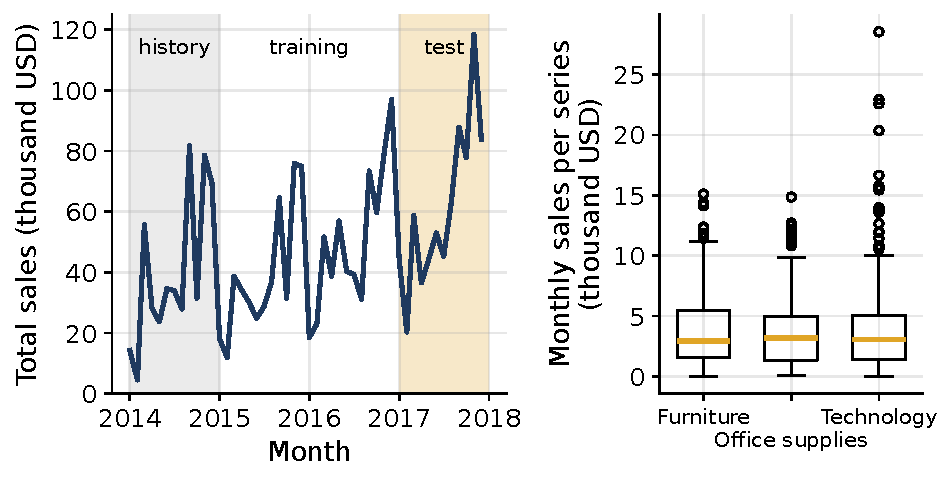
\includegraphics[width=\linewidth]{figures/eda_overview.pdf}
\caption{Izquierda: ventas mensuales totales de la empresa, con el año que solo aporta historia (2014), el periodo de entrenamiento (2015--2016) y el de prueba (2017). Derecha: distribución de las ventas mensuales por serie en cada categoría; los puntos son valores atípicos.}
\label{fig:eda}
\end{figure}

\begin{figure}[!htb]
\centering
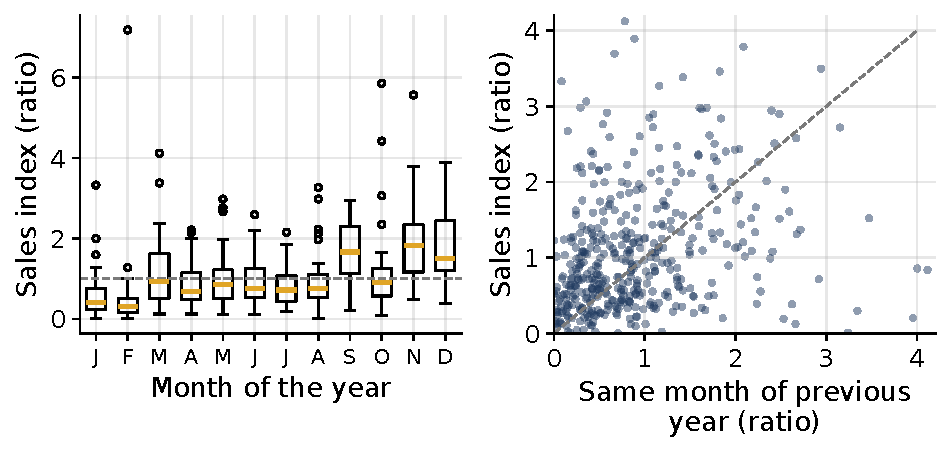
\includegraphics[width=\linewidth]{figures/eda_index.pdf}
\caption{Izquierda: distribución del índice de ventas por mes del año (2015--2017); la línea discontinua marca el nivel promedio de los doce meses previos. Derecha: índice de ventas frente a las ventas relativas del mismo mes del año anterior; la línea discontinua es la identidad.}
\label{fig:indice}
\end{figure}

\textbf{Decisiones derivadas del análisis exploratorio.} (i) La estacionalidad motiva el rezago de doce meses y la codificación cíclica del mes, que mantiene diciembre junto a enero. (ii) El crecimiento de 2016--2017 y la diferencia de escala entre series motivan el índice de la Ecuación~\eqref{eq:indice}: dividir por el nivel reciente hace comparables las series y elimina la tendencia de la variable objetivo. (iii) Los atípicos son ventas reales y se conservan; por eso la métrica primaria es el MAE y no el error cuadrático. (iv) Descuento, cantidad y utilidad no se conocen antes de que ocurra el mes y se excluyen para evitar fuga de información. (v) La débil relación con la historia reciente no justifica descartarla a priori; su aporte se evalúa en la ablación.

\subsection{Modelos de referencia (baselines)}\label{subsec:sota}

El modelo propuesto se compara con ocho referencias: el pronóstico ingenuo estacional y siete regresores que cubren familias lineales, bayesianas, de vecinos, de árboles y de núcleo. Todos predicen el índice $z$ a partir de las mismas variables, con el mismo preprocesamiento y la misma partición; sea $\mathcal{D}=\{(\mathbf{x}_i,z_i)\}_{i=1}^{n}$ la muestra de entrenamiento ya codificada.

El \textbf{ingenuo estacional} \cite{hyndman2021} no estima parámetros y representa la práctica actual de planificación:
\begin{equation}
\hat{y}_{s,t}=y_{s,t-12}.
\label{eq:naive}
\end{equation}
\textbf{Ridge} y \textbf{Lasso} ajustan un modelo lineal por mínimos cuadrados penalizados, con penalización $\ell_2$ y $\ell_1$ respectivamente \cite{hoerl1970,tibshirani1996}:
\begin{equation}
\hat{\boldsymbol{\beta}}=\arg\min_{\beta_0,\boldsymbol{\beta}}\sum_{i=1}^{n}\bigl(z_i-\beta_0-\mathbf{x}_i^{\top}\boldsymbol{\beta}\bigr)^2+\lambda R(\boldsymbol{\beta}),\qquad R(\boldsymbol{\beta})=\lVert\boldsymbol{\beta}\rVert_2^2\ \text{o}\ \lVert\boldsymbol{\beta}\rVert_1.
\label{eq:ridge}
\end{equation}
La \textbf{regresión bayesiana} (\texttt{BayesianRidge}) coloca una distribución a priori gaussiana sobre los coeficientes y estima las precisiones del ruido y de los pesos maximizando la verosimilitud marginal \cite{mackay1992}:
\begin{equation}
z_i\mid\mathbf{x}_i,\boldsymbol{\beta},\alpha\sim\mathcal{N}\bigl(\mathbf{x}_i^{\top}\boldsymbol{\beta},\alpha^{-1}\bigr),\qquad \boldsymbol{\beta}\mid\lambda\sim\mathcal{N}\bigl(\mathbf{0},\lambda^{-1}\mathbf{I}\bigr),
\label{eq:bayes}
\end{equation}
con distribuciones a priori Gamma sobre $\alpha$ y $\lambda$; el pronóstico es la media de la distribución predictiva. \textbf{KNN} promedia el índice de los $k$ vecinos más cercanos en distancia euclidiana \cite{cover1967}:
\begin{equation}
\hat{f}(\mathbf{x})=\frac{1}{k}\sum_{i\in\mathcal{N}_k(\mathbf{x})}z_i.
\label{eq:knn}
\end{equation}
El \textbf{árbol de decisión} particiona el espacio de variables de forma recursiva, eligiendo en cada nodo la variable $j$ y el umbral $u$ que minimizan la suma de cuadrados dentro de las dos regiones resultantes \cite{breiman1984}:
\begin{equation}
\min_{j,u}\Bigl[\sum_{i:\,x_{ij}\le u}\bigl(z_i-\bar{z}_{R_1}\bigr)^2+\sum_{i:\,x_{ij}>u}\bigl(z_i-\bar{z}_{R_2}\bigr)^2\Bigr].
\label{eq:arbol}
\end{equation}
\textbf{XGBoost} construye un ensamble aditivo de $M$ árboles, $\hat{z}_i=\sum_{m=1}^{M}f_m(\mathbf{x}_i)$, minimizando un objetivo regularizado \cite{chen2016}:
\begin{equation}
\mathcal{L}=\sum_{i=1}^{n}\bigl(z_i-\hat{z}_i\bigr)^2+\sum_{m=1}^{M}\Bigl(\gamma\,T_m+\tfrac{1}{2}\lambda\lVert\mathbf{w}_m\rVert_2^2\Bigr),
\label{eq:xgb}
\end{equation}
donde $T_m$ es el número de hojas del árbol $m$ y $\mathbf{w}_m$ sus pesos. La \textbf{regresión de vectores de soporte} (SVR) ajusta $f(\mathbf{x})=\mathbf{w}^{\top}\phi(\mathbf{x})+b$ bajo la pérdida insensible a $\varepsilon$ \cite{drucker1997}:
\begin{equation}
\min_{\mathbf{w},b}\ \tfrac{1}{2}\lVert\mathbf{w}\rVert_2^2+C\sum_{i=1}^{n}\max\bigl(0,\lvert z_i-f(\mathbf{x}_i)\rvert-\varepsilon\bigr),
\label{eq:svr}
\end{equation}
con núcleo gaussiano $K(\mathbf{x},\mathbf{x}')=\exp(-\gamma\lVert\mathbf{x}-\mathbf{x}'\rVert_2^2)$. Se usaron las implementaciones de scikit-learn 1.7.2 \cite{pedregosa2011} y XGBoost 3.2.0 \cite{chen2016}. La Tabla~\ref{tab:rejillas} lista las rejillas exploradas.

\begin{table}[!htb]
\caption{Rejillas de hiperparámetros exploradas con búsqueda exhaustiva y configuración seleccionada por validación cruzada temporal. Los demás hiperparámetros conservan los valores por defecto de la librería.}\label{tab:rejillas}
\footnotesize
\begin{tabular*}{\textwidth}{@{\extracolsep\fill}p{0.15\textwidth}p{0.44\textwidth}cp{0.25\textwidth}}
\toprule
Modelo & Rejilla & Config. & Seleccionada \\
\midrule
Ridge & $\alpha\in\{0.01, 0.1, 1, 10, 100\}$ & 5 & $\alpha=100$ \\
Lasso & $\alpha\in\{10^{-4}, 10^{-3}, 10^{-2}, 10^{-1}\}$ & 4 & $\alpha=10^{-2}$ \\
Reg. bayesiana & $\alpha_1,\lambda_1\in\{10^{-6}, 10^{-3}, 1\}$ & 9 & $\alpha_1=1$, $\lambda_1=10^{-6}$ \\
KNN & $k\in\{3, 5, 10, 15, 20, 30\}$; pesos uniformes o por distancia & 12 & $k=10$, uniformes \\
Árbol de decisión & profundidad $\in\{2, 3, 4, 6\}$; mín. por hoja $\in\{1, 5, 10, 20\}$ & 16 & profundidad 3, hoja 20 \\
XGBoost (300 árboles) & profundidad $\in\{2, 3, 4\}$; tasa $\in\{0.03, 0.1\}$; submuestra $\in\{0.8, 1\}$; peso mín. de hijo $\in\{1, 5\}$ & 24 & 2; 0.03; 0.8; 5 \\
SVR (núcleo RBF) & $C\in\{0.1, 1, 10\}$; $\varepsilon\in\{0.05, 0.1, 0.2\}$; $\gamma\in\{\text{scale}, 0.05\}$ & 18 & $C=1$, $\varepsilon=0.2$, scale \\
Random Forest (300 árboles) & profundidad $\in\{3, 5, \text{sin límite}\}$; mín. por hoja $\in\{1, 3, 5, 10\}$; fracción de variables $\in\{1, 0.5\}$ & 24 & 5; 3; 0.5 \\
\botrule
\end{tabular*}
\end{table}

\subsection{Modelo propuesto}\label{subsec:propuesto}

\textbf{Idea central.} El modelo propuesto es un Random Forest \emph{global}: un único Random Forest entrenado con las doce series agrupadas, que predice el índice libre de escala de la Ecuación~\eqref{eq:indice} y cuyo resultado se devuelve a dólares con la Ecuación~\eqref{eq:retorno}; para horizontes mayores a un mes se aplica de forma recursiva. La Figura~\ref{fig:metodo} muestra el flujo y el Algoritmo~\ref{alg:propuesto} el procedimiento.

\begin{figure}[!htb]
\centering
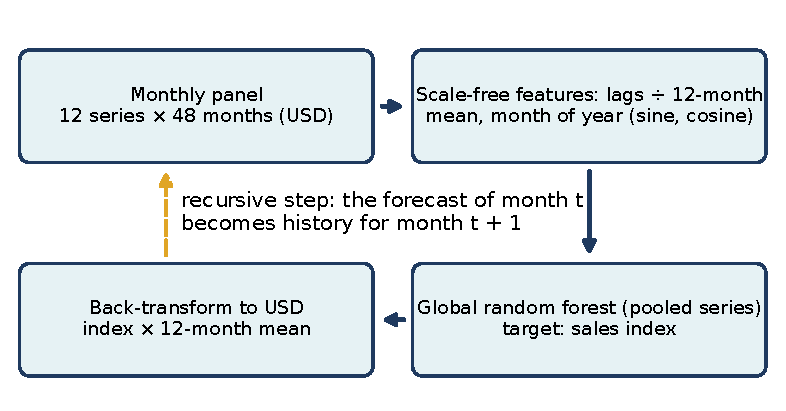
\includegraphics[width=\linewidth]{figures/method_diagram.pdf}
\caption{Flujo del modelo propuesto. El panel mensual en dólares se transforma en variables libres de escala, el Random Forest global predice el índice de ventas y el resultado se devuelve a dólares; en la proyección a varios meses, cada pronóstico se incorpora a la historia del mes siguiente.}
\label{fig:metodo}
\end{figure}

El Random Forest promedia $B$ árboles de regresión, cada uno crecido sobre una muestra \emph{bootstrap} y considerando en cada nodo un subconjunto aleatorio de variables \cite{breiman2001}:
\begin{equation}
\hat{f}(\mathbf{x})=\frac{1}{B}\sum_{b=1}^{B}T_b(\mathbf{x};\Theta_b),
\label{eq:rf}
\end{equation}
donde $\Theta_b$ reúne la muestra y las variables sorteadas para el árbol $b$, y cada árbol se construye con el criterio de la Ecuación~\eqref{eq:arbol}. Para un horizonte $h>1$, las ventas aún no observadas se sustituyen por sus pronósticos al calcular el nivel y los rezagos \cite{taieb2012}:
\begin{equation}
\hat{y}_{s,t+h}=\max\bigl(0,\;\hat{f}(\tilde{\mathbf{x}}_{s,t+h})\,\tilde{\ell}_{s,t+h}\bigr),\qquad \tilde{y}_{s,u}=\begin{cases}y_{s,u}, & u\le t,\\ \hat{y}_{s,u}, & u>t,\end{cases}
\label{eq:recursivo}
\end{equation}
con $\tilde{\mathbf{x}}$ y $\tilde{\ell}$ calculados sobre $\tilde{y}$.

\begin{algorithm}
\caption{Random Forest global sobre el índice de ventas y proyección recursiva}\label{alg:propuesto}
\begin{algorithmic}[1]
\Require Panel $\{y_{s,t}\}$ hasta el mes $t_0$, rejilla $\mathcal{G}$, número de árboles $B$, horizonte $H$
\Ensure Pronósticos $\hat{y}_{s,t_0+h}$ para $h=1,\dots,H$ y toda serie $s$
\State Calcular $\ell_{s,t}$, $z_{s,t}$ y $\mathbf{x}_{s,t}$ con las Ecuaciones~\eqref{eq:indice} y \eqref{eq:x} para todo $t\le t_0$ con doce meses de historia
\For{cada configuración $g\in\mathcal{G}$}
    \State Estimar el MAE del índice con validación cruzada temporal de 4 pliegues
\EndFor
\State Ajustar el Random Forest $\hat{f}$ de $B$ árboles con la configuración de menor MAE sobre las series agrupadas
\For{$h=1,\dots,H$}
    \State Calcular $\tilde{\ell}_{s,t_0+h}$ y $\tilde{\mathbf{x}}_{s,t_0+h}$ con la historia observada y los pronósticos previos
    \State $\hat{y}_{s,t_0+h}\gets\max\bigl(0,\hat{f}(\tilde{\mathbf{x}}_{s,t_0+h})\,\tilde{\ell}_{s,t_0+h}\bigr)$
    \State Añadir $\hat{y}_{s,t_0+h}$ a la historia de la serie $s$
\EndFor
\State \Return $\{\hat{y}_{s,t_0+h}\}$
\end{algorithmic}
\end{algorithm}

\textbf{Justificación de cada componente.} (a) \emph{Índice libre de escala:} los árboles predicen promedios de valores vistos en entrenamiento y no pueden extrapolar; con ventas que crecieron 20--30\% anual, un objetivo en dólares quedaría acotado por el nivel de 2015--2016. El índice traslada la tendencia al nivel $\ell_{s,t}$, que se actualiza cada mes, y deja al modelo la parte estacionaria, como hacen los métodos globales que normalizan por la escala de la serie \cite{salinas2020,smyl2020}. (b) \emph{Modelo global:} cada serie aporta solo 24 meses de entrenamiento; agruparlas multiplica por doce la muestra y es razonable cuando las series comparten estacionalidad \cite{monteromanso2021}. Categoría y región entran como variables para permitir diferencias entre series. (c) \emph{Rezago estacional y codificación cíclica:} capturan la estacionalidad observada en el análisis exploratorio desde dos ángulos, el patrón propio de la serie y el patrón común del calendario. (d) \emph{Historia reciente:} el mes anterior y el promedio trimestral permiten corregir desviaciones de corto plazo. (e) \emph{Random Forest:} el promedio de árboles decorrelacionados reduce la varianza \cite{breiman2001}, deseable con 288 observaciones ruidosas, y captura interacciones entre el mes y los rezagos sin especificarlas.

\textbf{Complejidad.} El entrenamiento cuesta $\mathcal{O}(B\,p'\,n\log n)$ en tiempo, con $B=300$, $n=288$ y $p'=6$ de las 12 columnas codificadas consideradas por nodo, y la predicción $\mathcal{O}(B\,D)$ por observación, con profundidad $D\le5$. El modelo no tiene parámetros entrenados por gradiente; su tamaño lo determinan los nodos de los árboles (en promedio 37.9 por árbol, unos 11{,}400 en total).

\textbf{Qué es nuevo y qué se reutiliza.} Ninguno de los componentes es original por separado: el Random Forest \cite{breiman2001}, el entrenamiento global \cite{monteromanso2021}, la normalización por nivel \cite{salinas2020,smyl2020} y la estrategia recursiva \cite{taieb2012} provienen de la literatura. El aporte es su combinación en una formulación de regresión reproducible para paneles minoristas pequeños y, sobre todo, su evaluación con un protocolo estadístico y un estudio de ablación que aísla el efecto de cada componente.

\subsection{Entrenamiento y optimización}\label{subsec:entrenamiento}

Los hiperparámetros de todos los modelos se ajustaron con búsqueda exhaustiva en rejilla (\texttt{GridSearchCV}) sobre los datos de 2015--2016, con validación cruzada temporal (\texttt{TimeSeriesSplit}) de 4 pliegues: cada pliegue valida con los tres meses siguientes a su ventana de entrenamiento (36 filas), de modo que los cuatro pliegues recorren los trimestres de 2016 con ventanas crecientes de 144, 180, 216 y 252 filas. El criterio es el MAE del índice, Ecuación~\eqref{eq:perdida}. El codificador y el escalador se reajustan dentro de cada pliegue. Las rejillas tienen entre 4 y 24 configuraciones (Tabla~\ref{tab:rejillas}); el modelo propuesto recibió 24, igual que XGBoost, y ningún modelo usó valores por defecto sin búsqueda, de modo que el presupuesto de ajuste es comparable. No hay épocas, tasa de aprendizaje ni parada temprana en el modelo propuesto; el Random Forest usa 300 árboles, muestreo \emph{bootstrap} y semilla 42. Tras la selección, cada modelo se reajusta con todo el periodo de entrenamiento. El conjunto de prueba no interviene en ninguna decisión: el modelo propuesto se identificó como el de menor MAE de validación cruzada antes de evaluar 2017.

\subsection{Protocolo de evaluación}\label{subsec:evaluacion}

\textbf{Métricas.} La métrica primaria es el MAE en dólares por serie y mes sobre 2017, con pronósticos a un paso: el modelo queda fijo con datos hasta diciembre de 2016 y sus variables usan las ventas observadas hasta el mes anterior. Las métricas secundarias son la raíz del error cuadrático medio (RMSE), el error porcentual absoluto ponderado (WAPE), el error absoluto escalado (MASE) \cite{hyndman2006}, el coeficiente $R^2$ y el desvío del total anual:
\begin{gather}
\mathrm{WAPE}=\frac{\sum_{s,t}\lvert e_{s,t}\rvert}{\sum_{s,t}y_{s,t}},\qquad
\Delta_{\mathrm{total}}=\frac{\sum_{s,t}\hat{y}_{s,t}}{\sum_{s,t}y_{s,t}}-1,\notag\\
\mathrm{MASE}=\frac{\frac{1}{n_{\mathrm{te}}}\sum_{s,t\in\mathrm{prueba}}\lvert e_{s,t}\rvert}{\frac{1}{n}\sum_{s,t\in\mathrm{entr.}}\lvert y_{s,t}-y_{s,t-12}\rvert}.
\label{eq:metricas}
\end{gather}
Se usa WAPE en lugar de MAPE porque hay meses con ventas cercanas a cero que vuelven inestable el error porcentual individual. Como la aplicación es una proyección anual, se añade una \emph{prueba recursiva a doce meses}: con el Algoritmo~\ref{alg:propuesto} y datos hasta 2016 se proyecta todo 2017 y se reportan el MAE y el desvío del total.

\textbf{Incertidumbre.} Con una sola serie temporal de evaluación no hay pliegues intercambiables. La variabilidad se reporta como media $\pm$ desviación estándar del MAE sobre los doce bloques mensuales de prueba (12 series cada uno), como desviación entre diez semillas para los modelos con componente aleatorio, y con intervalos de confianza del 95\% por \emph{bootstrap} de bloques móviles circulares \cite{kunsch1989} de tres meses y 10{,}000 remuestras.

\textbf{Pruebas de significancia.} Se sigue la combinación recomendada para pronóstico de series de tiempo \cite{cerqueira2020}; la prueba $t$ con varianza corregida \cite{nadeau2003} no se usa porque supone particiones intercambiables. Para cada referencia $b$ se define el diferencial de pérdida absoluta promediado sobre las series, lo que absorbe la dependencia entre series de un mismo mes:
\begin{equation}
d_t=\frac{1}{S}\sum_{s=1}^{S}\bigl(\lvert e^{\mathrm{prop}}_{s,t}\rvert-\lvert e^{b}_{s,t}\rvert\bigr),\qquad t=1,\dots,12,
\label{eq:dt}
\end{equation}
con valores negativos a favor del modelo propuesto. (1) La prueba de \emph{Diebold--Mariano} \cite{diebold1995} con la corrección de Harvey--Leybourne--Newbold \cite{harvey1997} contrasta $\mathbb{E}[d_t]=0$ con el estadístico $\sqrt{(T-1)/T}\;\bar{d}/\sqrt{\hat{\gamma}_0/T}$ para horizonte 1, comparado con una $t_{T-1}$; se repite con pérdida cuadrática como comprobación. (2) La prueba de \emph{Giacomini--White} \cite{giacomini2006} de capacidad predictiva condicional usa los instrumentos $\mathbf{h}_t=(1,d_t)^{\top}$ y el estadístico $n\,\bar{\mathbf{Z}}^{\top}\hat{\boldsymbol{\Omega}}^{-1}\bar{\mathbf{Z}}\sim\chi^2_2$, con $\mathbf{Z}_{t+1}=\mathbf{h}_t d_{t+1}$ y $n=11$. (3) La prueba $t$ \emph{correlacionada bayesiana} \cite{corani2015,benavoli2017} sobre el MAE mensual estima la probabilidad posterior de que el modelo propuesto sea mejor, equivalente o peor respecto de una región de equivalencia práctica (ROPE) de $\pm1$\% de la venta media de entrenamiento ($\pm37.49$ USD), con correlación $\rho=1/12$; por la dependencia temporal se interpreta con cautela. Cuando las diferencias mensuales no son aproximadamente normales (Shapiro--Wilk) se añade la prueba de rangos con signo de Wilcoxon. Los valores $p$ de los $m=8$ contrastes se ajustan con el método de Holm \cite{holm1979} por separado para cada prueba, con $\alpha=0.05$. Cada contraste se acompaña de la diferencia media de MAE con su intervalo de confianza y de la $d$ de Cohen de las diferencias pareadas. La prueba de Friedman no se aplica porque hay un solo conjunto de datos.

\textbf{Registro del protocolo.} La partición, la métrica primaria y la regla de selección estaban fijadas en el código antes de evaluar 2017. Las pruebas de significancia se especificaron después de conocer las métricas agregadas de prueba, tomando la combinación estándar para pronóstico sin variar pruebas, pérdidas, semillas ni particiones en función del resultado; los análisis no previstos se marcan como exploratorios.

\subsection{Diseño del estudio de ablación}\label{subsec:ablacion}

Cada variante elimina o reemplaza un componente del modelo completo y mantiene lo demás: misma rejilla, misma validación cruzada, mismas métricas y mismas pruebas. Las hipótesis son: (H1) \emph{sin codificación del mes}: el error aumenta porque se pierde el patrón de calendario común; (H2) \emph{sin rezago estacional}: el error aumenta porque se pierde el patrón propio de la serie; (H3) \emph{sin historia reciente}: el error aumenta poco, dado su débil vínculo con el índice; (H4) \emph{sin identificadores de serie}: el error aumenta si las series difieren más allá de su escala; (H5) \emph{sin índice}, con objetivo y rezagos en dólares: el error aumenta y el total se subestima, porque los árboles no extrapolan el crecimiento; (H6) \emph{sin modelo global}, con un Random Forest por serie (24 observaciones cada uno): el error aumenta por falta de datos.

\subsection{Configuración experimental y disponibilidad}\label{subsec:config}

Los experimentos se ejecutaron en un computador portátil con procesador AMD Ryzen 5 7520U (4 núcleos, 8 hilos), 8 GB de memoria RAM y Windows 11, sin GPU, con Python 3.10.11, scikit-learn 1.7.2, XGBoost 3.2.0, pandas 2.3.3, NumPy 2.2.6, SciPy 1.15.3 y statsmodels 0.15.0. Se midieron tres tiempos: la búsqueda completa en rejilla (en paralelo), el reajuste de la configuración seleccionada (mediana de 5 repeticiones, un hilo) y la predicción de las 144 filas de prueba (mediana de 30 repeticiones); como indicador de memoria se reporta el tamaño del modelo serializado. La semilla es 42 para los modelos y el \emph{bootstrap}, y $\{0,\dots,9\}$ en el análisis de semillas. El código, los datos y las versiones exactas de las librerías están en el repositorio indicado en las Declaraciones; el script \texttt{paper/experimentos.py} reproduce todas las tablas, pruebas y figuras de este artículo.

\section{Resultados}\label{sec:resultados}

\subsection{Resumen del montaje experimental}\label{subsec:montaje}

Se evalúan nueve métodos sobre las 144 observaciones de 2017 (12 series por 12 meses), con modelos ajustados con 2015--2016 e hiperparámetros elegidos por validación cruzada temporal. La métrica primaria es el MAE en dólares a un paso; las secundarias son RMSE, WAPE, MASE, $R^2$, el desvío del total anual y la prueba recursiva a doce meses. La incertidumbre se mide sobre doce bloques mensuales y diez semillas.

\subsection{Desempeño predictivo global}\label{subsec:global}

La Tabla~\ref{tab:resultados} resume el desempeño. El modelo propuesto reduce el MAE del ingenuo estacional en 278 USD por serie y mes (9.5\%) y el RMSE en 15.1\%, y es el de menor variabilidad entre meses. Frente a los demás regresores las diferencias son pequeñas: los ocho métodos entrenados quedan en una franja de 246 USD de MAE, menos de un tercio de la desviación entre bloques mensuales de cualquiera de ellos (Figura~\ref{fig:box}). El modelo propuesto no es el mejor en ninguna columna: ocupa el segundo lugar en MAE (y en sus reescalados WAPE y MASE), RMSE, $R^2$ y en ambos desvíos del total, y el tercero en MAE recursivo. SVR obtiene el menor MAE, 123 USD por debajo del propuesto (4.7\%), pero subestima el total anual en 13.8\%, casi tanto como el ingenuo estacional ($-16.9$\%), mientras que el modelo propuesto lo desvía en $+0.7$\% a un paso y en $+3.4$\% en la proyección recursiva.

\begin{table}[!htb]
\caption{Desempeño en el conjunto de prueba (2017, 144 observaciones). MAE: media $\pm$ desviación estándar sobre los doce bloques mensuales. $\Delta_1$ y $\Delta_{12}$: desvío del total anual con pronósticos a un paso y con proyección recursiva a doce meses; MAE$_{12}$: MAE de la proyección recursiva. En negrita el mejor valor de cada columna y subrayado el segundo.}\label{tab:resultados}
\footnotesize
\begin{tabular*}{\textwidth}{@{\extracolsep\fill}lrrrrrrrr}
\toprule
Modelo & MAE (USD) & RMSE & WAPE (\%) & MASE & $R^2$ & $\Delta_1$ (\%) & MAE$_{12}$ & $\Delta_{12}$ (\%) \\
\midrule
Ingenuo estacional & 2{,}912 $\pm$ 911 & 4{,}379 & 57.2 & 1.198 & $-0.107$ & $-16.9$ & 2{,}912 & $-16.9$ \\
Ridge & 2{,}708 $\pm$ 962 & 3{,}727 & 53.2 & 1.114 & 0.198 & $-1.6$ & 2{,}671 & $+4.1$ \\
Lasso & 2{,}698 $\pm$ 983 & \textbf{3{,}707} & 53.0 & 1.110 & \textbf{0.206} & $-1.6$ & 2{,}633 & $\mathbf{+2.9}$ \\
Regresión bayesiana & 2{,}709 $\pm$ 959 & 3{,}728 & 53.2 & 1.114 & 0.198 & $-1.6$ & 2{,}674 & $+4.4$ \\
KNN & 2{,}757 $\pm$ 1{,}128 & 3{,}890 & 54.2 & 1.134 & 0.126 & $+2.2$ & 2{,}933 & $+11.1$ \\
Árbol de decisión & 2{,}635 $\pm$ 973 & 3{,}726 & 51.8 & 1.084 & 0.198 & $\mathbf{+0.6}$ & \underline{2{,}537} & $+3.5$ \\
XGBoost & 2{,}672 $\pm$ 906 & 3{,}797 & 52.5 & 1.099 & 0.168 & $+1.7$ & 2{,}908 & $+10.4$ \\
SVR & \textbf{2{,}511} $\pm$ 1{,}017 & 3{,}775 & \textbf{49.3} & \textbf{1.033} & 0.177 & $-13.8$ & \textbf{2{,}370} & $-13.8$ \\
Modelo propuesto & \underline{2{,}634} $\pm$ 834 & \underline{3{,}719} & \underline{51.7} & \underline{1.083} & \underline{0.201} & \underline{$+0.7$} & 2{,}609 & \underline{$+3.4$} \\
\botrule
\end{tabular*}
\footnotetext{Ninguna diferencia entre el modelo propuesto y las referencias es significativa tras la corrección de Holm (Tabla~\ref{tab:pruebas}), por lo que no se añaden símbolos de significancia.}
\end{table}

\begin{figure}[!htb]
\centering
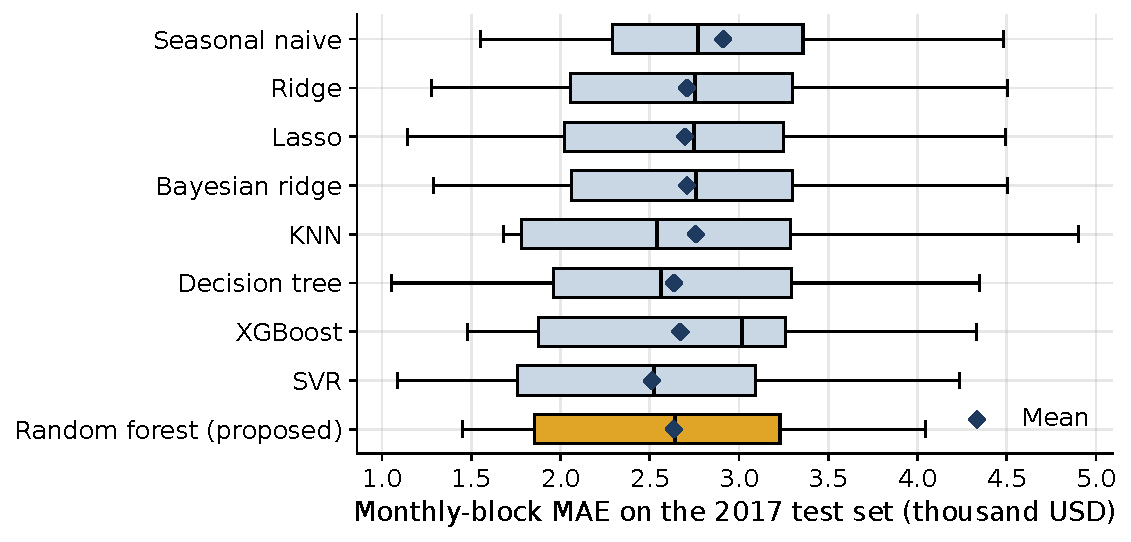
\includegraphics[width=\linewidth]{figures/mae_boxplot.pdf}
\caption{Distribución del MAE de los doce bloques mensuales de prueba para cada modelo. El rombo indica la media, que coincide con el MAE global de la Tabla~\ref{tab:resultados}.}
\label{fig:box}
\end{figure}

Todos los MASE superan 1 porque el denominador se calcula en 2015--2016, cuando las ventas eran menores; la comparación relevante es entre filas. El $R^2$ de 0.20 indica que, a nivel de serie y mes, el modelo explica una fracción pequeña de la variabilidad: la Figura~\ref{fig:pred} muestra predicciones concentradas entre 2{,}000 y 10{,}000 USD frente a observaciones que alcanzan 23{,}000 USD. El desempeño mejora al agregar: sobre el total mensual de la empresa el WAPE baja a 19.3\% a un paso y a 17.7\% en la proyección recursiva, frente a 25.3\% del ingenuo estacional, y la Figura~\ref{fig:serie} muestra que el modelo sigue el perfil del año salvo en el cierre.

\begin{figure}[!htb]
\centering
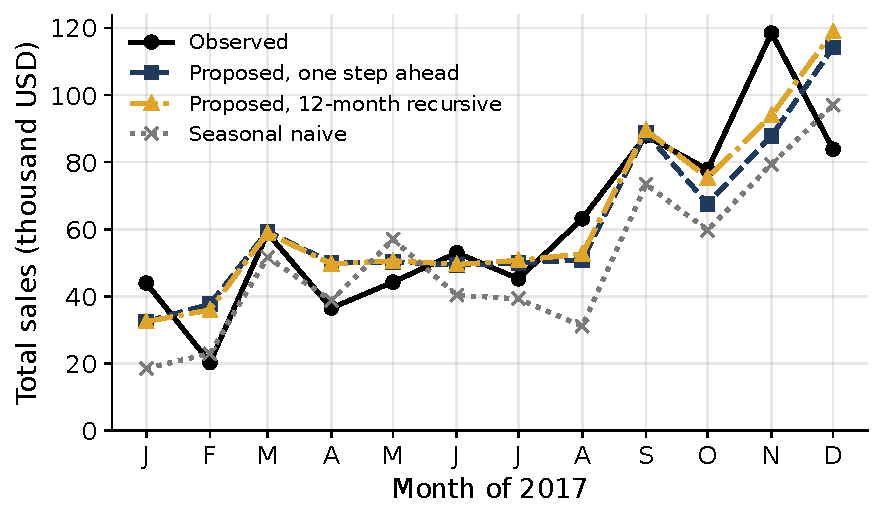
\includegraphics[width=\linewidth]{figures/forecast_total.pdf}
\caption{Ventas totales mensuales de 2017: observadas, pronosticadas por el modelo propuesto a un paso y con proyección recursiva a doce meses, y pronóstico ingenuo estacional.}
\label{fig:serie}
\end{figure}

\begin{figure}[!htb]
\centering
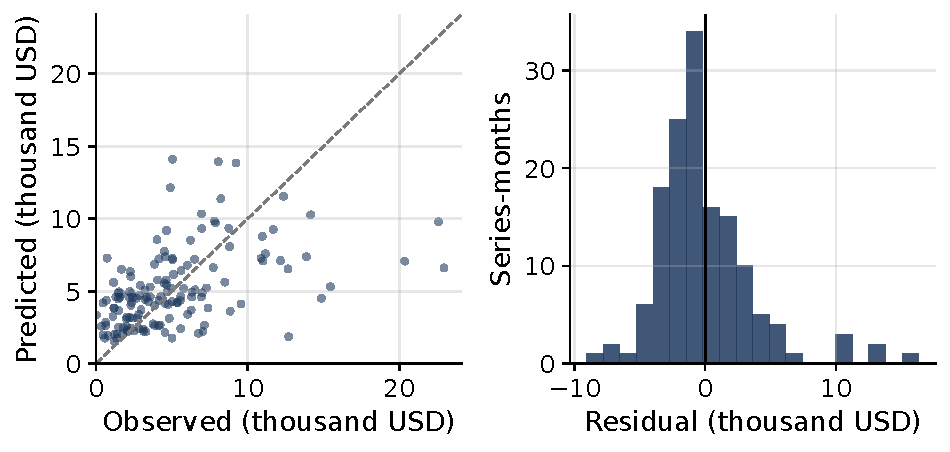
\includegraphics[width=\linewidth]{figures/pred_vs_obs.pdf}
\caption{Modelo propuesto en el conjunto de prueba. Izquierda: ventas pronosticadas frente a observadas por serie y mes; la línea discontinua es la identidad. Derecha: distribución de los residuos (observado menos pronosticado).}
\label{fig:pred}
\end{figure}

\subsection{Resultados de las pruebas de significancia}\label{subsec:pruebas}

La Tabla~\ref{tab:pruebas} y la Figura~\ref{fig:dif} presentan los contrastes. El modelo propuesto no supera significativamente a ninguna de las 8 referencias ($p_{\mathrm{Holm}}\ge0.555$ en las pruebas de Diebold--Mariano y Giacomini--White) y es estadísticamente indistinguible de las 8, incluida SVR, cuyo menor MAE tampoco constituye evidencia de diferencia ($p=0.484$ sin ajustar). Los intervalos de confianza de la diferencia de MAE contienen el cero en todos los casos.

\begin{table}[!htb]
\caption{Contrastes del modelo propuesto frente a cada referencia en el conjunto de prueba ($T=12$ bloques mensuales). $\Delta$MAE: diferencia media propuesto menos referencia, en USD, con intervalo de confianza del 95\% por \emph{bootstrap} de bloques (valores negativos favorecen al propuesto). $d$: $d$ de Cohen de las diferencias pareadas. DM: Diebold--Mariano con corrección HLN y pérdida absoluta; GW: Giacomini--White; entre paréntesis, valor $p$ sin ajustar y ajustado por Holm ($m=8$). Bayes: probabilidad posterior de que el propuesto sea mejor / equivalente dentro de la ROPE / peor.}\label{tab:pruebas}
\scriptsize
\begin{tabular*}{\textwidth}{@{\extracolsep\fill}lrrrrr}
\toprule
Referencia & $\Delta$MAE [IC 95\%] & $d$ & DM ($p$; $p_{\mathrm{Holm}}$) & GW ($p$; $p_{\mathrm{Holm}}$) & Bayes \\
\midrule
Ingenuo estacional & $-278$ [$-638$, 56] & $-0.40$ & $-1.39$ (0.191; 1.000) & 1.82 (0.403; 1.000) & 0.79 / 0.06 / 0.15 \\
Ridge & $-74$ [$-247$, 104] & $-0.13$ & $-0.44$ (0.671; 1.000) & 5.30 (0.071; 0.555) & 0.56 / 0.11 / 0.33 \\
Lasso & $-63$ [$-248$, 125] & $-0.10$ & $-0.35$ (0.731; 1.000) & 1.69 (0.430; 1.000) & 0.54 / 0.11 / 0.35 \\
Regresión bayesiana & $-75$ [$-247$, 99] & $-0.13$ & $-0.44$ (0.667; 1.000) & 5.34 (0.069; 0.555) & 0.56 / 0.11 / 0.33 \\
KNN & $-123$ [$-371$, 118] & $-0.21$ & $-0.73$ (0.482; 1.000) & 0.13 (0.937; 1.000) & 0.63 / 0.10 / 0.26 \\
Árbol de decisión & $-1$ [$-128$, 110] & $-0.00$ & $-0.02$ (0.988; 1.000) & 0.14 (0.934; 1.000) & 0.37 / 0.28 / 0.36 \\
XGBoost & $-38$ [$-231$, 123] & $-0.15$ & $-0.53$ (0.604; 1.000) & 4.18 (0.124; 0.743) & 0.50 / 0.26 / 0.24 \\
SVR & $+123$ [$-139$, 409] & $+0.21$ & $+0.72$ (0.484; 1.000) & 0.79 (0.675; 1.000) & 0.26 / 0.10 / 0.63 \\
\botrule
\end{tabular*}
\end{table}

\begin{figure}[!htb]
\centering
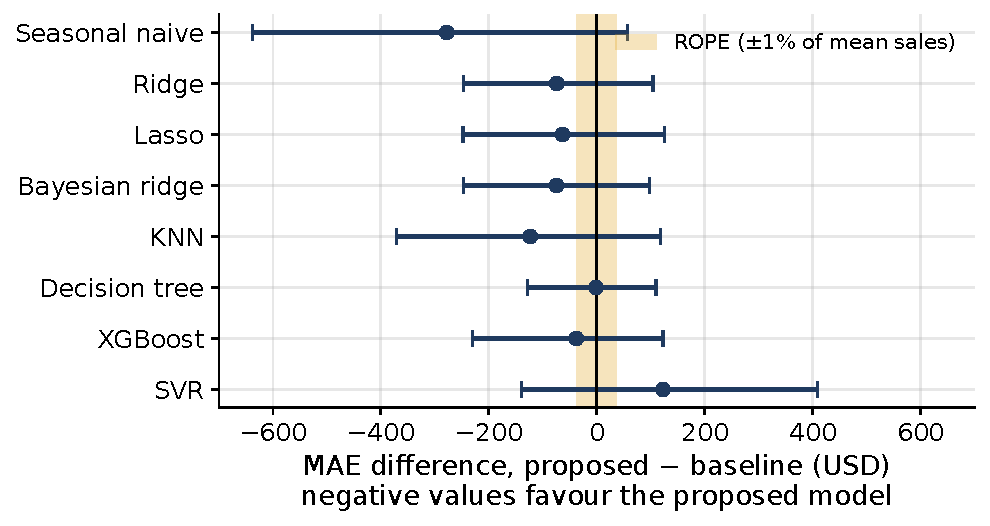
\includegraphics[width=\linewidth]{figures/mae_differences.pdf}
\caption{Diferencia media de MAE entre el modelo propuesto y cada referencia, con intervalo de confianza del 95\% por \emph{bootstrap} de bloques. La franja sombreada es la región de equivalencia práctica ($\pm1$\% de la venta media de entrenamiento).}
\label{fig:dif}
\end{figure}

El contraste más favorable es contra el ingenuo estacional: la diferencia es la mayor en magnitud, con un tamaño de efecto entre pequeño y mediano ($d=-0.40$) y una probabilidad posterior de 0.79 de que el modelo propuesto sea mejor. Con pérdida cuadrática, que pondera más los errores grandes del ingenuo, la prueba de Diebold--Mariano arroja $p=0.053$ sin ajustar, pero $p_{\mathrm{Holm}}=0.425$. La lectura correcta es que hay indicios, no evidencia concluyente, de mejora sobre la práctica actual. Frente a los regresores lineales, KNN y XGBoost las diferencias favorecen al propuesto pero con efectos pequeños ($\lvert d\rvert\le0.21$) y probabilidades posteriores entre 0.50 y 0.63; frente al árbol de decisión la diferencia es de 1 USD.

Las pruebas coinciden en la conclusión, aunque difieren en matices. Giacomini--White produce sus valores $p$ más bajos frente a Ridge y regresión bayesiana (0.071 y 0.069 sin ajustar) aun cuando Diebold--Mariano no detecta nada: su hipótesis es condicional y es sensible a que el diferencial dependa del mes anterior, no solo a una diferencia promedio. La prueba bayesiana asigna poca masa a la ROPE (0.06 a 0.28), lo que no significa que las diferencias sean relevantes sino que doce bloques no bastan para concentrar la distribución posterior. Las diferencias mensuales no son normales frente a Ridge, Lasso, regresión bayesiana y SVR (Shapiro--Wilk, $p<0.05$); la prueba de Wilcoxon, añadida como comprobación, tampoco rechaza en ningún caso ($p\ge0.176$ sin ajustar; $p_{\mathrm{Holm}}=1.000$).

Dos análisis posteriores al protocolo se reportan como \emph{exploratorios}. En la proyección recursiva a doce meses, los intervalos de la diferencia de MAE excluyen el cero a favor del modelo propuesto frente a KNN ($-324$ USD; [$-534$, $-141$]) y XGBoost ($-299$; [$-559$, $-106$]), y en su contra frente a SVR ($+239$; [61, 462]) y al árbol de decisión ($+72$; [8, 158]). Sobre el total mensual de la empresa, el sesgo medio del modelo propuesto es de $+418$ USD con un intervalo que contiene el cero ([$-6{,}688$, 7{,}341]), mientras que los del ingenuo estacional ($-10{,}334$; [$-19{,}199$, $-1{,}440$]) y de SVR ($-8{,}453$; [$-14{,}276$, $-2{,}871$]) son negativos con intervalos que lo excluyen.

\subsection{Resultados del estudio de ablación}\label{subsec:res_ablacion}

La Tabla~\ref{tab:ablacion} y la Figura~\ref{fig:abl} muestran las variantes. Ninguna difiere significativamente del modelo completo en MAE a un paso ($p_{\mathrm{Holm}}\ge0.563$ con Diebold--Mariano y $\ge0.886$ con Giacomini--White), por lo que las hipótesis se valoran por la dirección y magnitud del efecto.

\begin{table}[!htb]
\caption{Estudio de ablación sobre el conjunto de prueba. $\Delta$MAE: modelo completo menos variante, en USD, con intervalo de confianza del 95\% (valores negativos indican que quitar el componente empeora). $p_{\mathrm{Holm}}$: Diebold--Mariano con corrección HLN ($m=6$). Bayes: probabilidad posterior de que el modelo completo sea mejor / equivalente / peor. $\Delta_1$, MAE$_{12}$ y $\Delta_{12}$ como en la Tabla~\ref{tab:resultados}.}\label{tab:ablacion}
\scriptsize
\begin{tabular*}{\textwidth}{@{\extracolsep\fill}lrrrrrrr}
\toprule
Variante & MAE (USD) & $\Delta$MAE [IC 95\%] & $p_{\mathrm{Holm}}$ & Bayes & $\Delta_1$ (\%) & MAE$_{12}$ & $\Delta_{12}$ (\%) \\
\midrule
Modelo completo & 2{,}634 $\pm$ 834 & -- & -- & -- & $+0.7$ & 2{,}609 & $+3.4$ \\
Sin codificación del mes (H1) & 2{,}631 $\pm$ 876 & $+3$ [$-219$, 288] & 1.000 & 0.44 / 0.12 / 0.45 & $-0.8$ & 2{,}913 & $+15.2$ \\
Sin rezago estacional (H2) & 2{,}721 $\pm$ 1{,}055 & $-87$ [$-317$, 65] & 1.000 & 0.65 / 0.18 / 0.17 & $+0.5$ & 2{,}605 & $+2.9$ \\
Sin historia reciente (H3) & 2{,}629 $\pm$ 873 & $+5$ [$-71$, 74] & 1.000 & 0.30 / 0.35 / 0.35 & $+0.7$ & 2{,}636 & $+1.3$ \\
Sin identificadores (H4) & 2{,}688 $\pm$ 808 & $-54$ [$-180$, 49] & 1.000 & 0.57 / 0.26 / 0.17 & $+1.4$ & 2{,}708 & $+5.5$ \\
Sin índice, en dólares (H5) & 2{,}409 $\pm$ 895 & $+225$ [51, 412] & 0.563 & 0.08 / 0.07 / 0.84 & $-18.1$ & 2{,}317 & $-19.5$ \\
Sin modelo global (H6) & 2{,}690 $\pm$ 763 & $-56$ [$-299$, 239] & 1.000 & 0.53 / 0.11 / 0.36 & $-1.2$ & 2{,}829 & $+4.8$ \\
\botrule
\end{tabular*}
\end{table}

\begin{figure}[!htb]
\centering
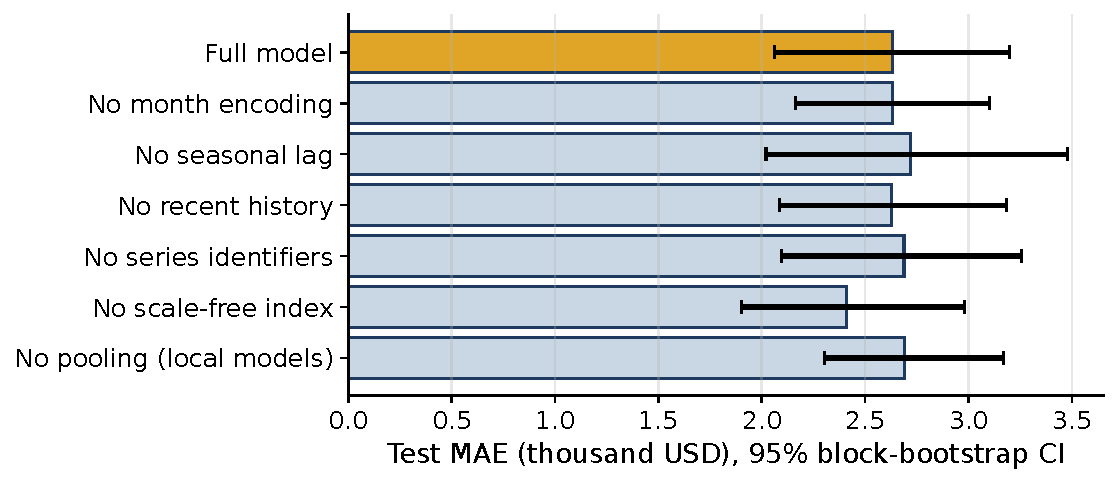
\includegraphics[width=\linewidth]{figures/ablation.pdf}
\caption{MAE de prueba del modelo completo y de cada variante de la ablación, con intervalos de confianza del 95\% por \emph{bootstrap} de bloques.}
\label{fig:abl}
\end{figure}

\emph{H1 (codificación del mes)} no se confirma a un paso, donde la variante iguala al modelo completo, pero sí en la proyección recursiva: sin el calendario el MAE sube a 2{,}913 USD y el total se sobrestima en 15.2\%, porque los errores se propagan sin un ancla estacional. \emph{H2 (rezago estacional)} recibe apoyo débil: quitarlo aumenta el MAE en 87 USD y la variabilidad entre meses, con probabilidad posterior de 0.65 a favor del modelo completo. \emph{H3 (historia reciente)} se confirma en su versión modesta: el componente no aporta (5 USD de diferencia; la mayor masa en la ROPE, 0.35) y podría eliminarse sin pérdida. \emph{H4 (identificadores)} y \emph{H6 (modelo global)} van en la dirección esperada, con efectos pequeños a un paso (54 y 56 USD); el modelo local empeora más en la proyección recursiva (2{,}829 USD).

\emph{H5 (índice)} se refuta en su primera parte y se confirma en la segunda. El Random Forest entrenado en dólares obtiene un MAE \emph{menor} que el modelo completo (225 USD; intervalo [51, 412], que excluye el cero aunque $p_{\mathrm{Holm}}=0.563$), pero subestima el total anual en 18.1\% a un paso y en 19.5\% en la proyección recursiva. El índice no mejora el error por serie: cambia errores absolutos algo mayores por un pronóstico sin sesgo de nivel. El mismo intercambio aparece entre el modelo propuesto y SVR en la Tabla~\ref{tab:resultados}.

\subsection{Sensibilidad y robustez}\label{subsec:sensibilidad}

\textbf{Semillas.} Con diez semillas, el MAE de prueba del modelo propuesto es 2{,}650 $\pm$ 12 USD (rango 2{,}633--2{,}670) y el de XGBoost 2{,}691 $\pm$ 20 USD; el árbol de decisión es determinista. La variación por semilla es unas 70 veces menor que la variación entre meses, de modo que la incertidumbre proviene de los datos y no del algoritmo, y la semilla 42 del experimento principal cae en el extremo favorable del rango.

\textbf{Hiperparámetros.} El MAE de validación cruzada del Random Forest varía entre 0.610 y 0.648 en las 24 configuraciones (Figura~\ref{fig:sens}, izquierda), con desviaciones entre pliegues cercanas a 0.11, mayores que cualquier diferencia entre configuraciones. Las peores son las de árboles sin restricción de profundidad con una observación por hoja. Evaluadas a posteriori sobre la prueba, solo con fines descriptivos, las 24 configuraciones dan MAE entre 2{,}583 y 2{,}861 USD; la seleccionada (2{,}634 USD) no es la mejor en prueba, como cabe esperar de una selección que no usa esos datos.

\textbf{Tamaño de entrenamiento.} La Figura~\ref{fig:sens} (derecha) muestra el MAE de prueba al entrenar solo con los últimos $k$ meses. Con 6 meses el error es 3{,}438 USD y con 12 meses 2{,}941 USD, ambos peores que el ingenuo estacional; el modelo solo lo supera a partir de 15 meses y la curva sigue descendiendo a los 24 meses. La cantidad de historia es, por tanto, un límite activo del desempeño.

\begin{figure}[!htb]
\centering
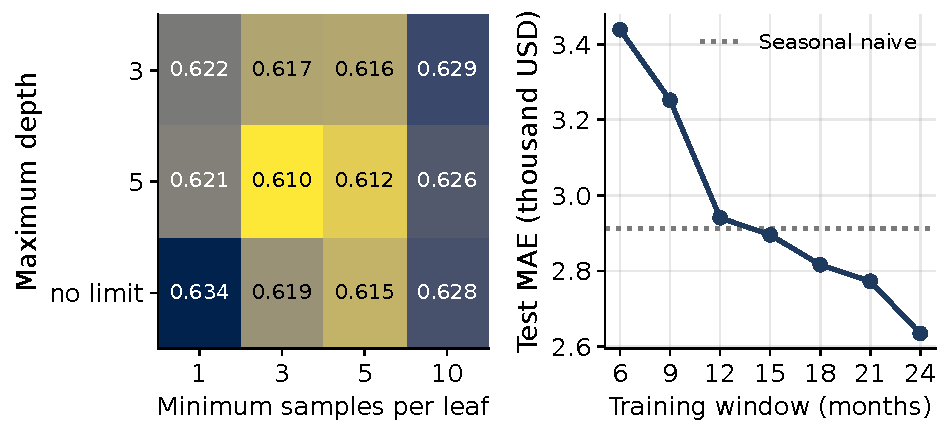
\includegraphics[width=\linewidth]{figures/sensitivity.pdf}
\caption{Izquierda: MAE de validación cruzada (sobre el índice) del Random Forest según la profundidad máxima y el mínimo de observaciones por hoja, con la mitad de las variables consideradas por nodo. Derecha: MAE de prueba según el número de meses de entrenamiento, con los hiperparámetros seleccionados fijos; la línea punteada es el ingenuo estacional.}
\label{fig:sens}
\end{figure}

\subsection{Costo computacional}\label{subsec:costo}

La Tabla~\ref{tab:costo} reporta el costo. El modelo propuesto es el más costoso en todas las dimensiones: su reajuste tarda 364 ms, entre 40 y 60 veces más que los modelos lineales, KNN, el árbol y SVR, y unas 7 veces más que XGBoost; predecir las 144 filas toma 17 ms frente a 3--6 ms, y el modelo serializado ocupa 874 kB. En términos absolutos el costo es irrelevante para una proyección que se actualiza una vez al mes, pero el resultado es claro: la reducción de error frente al árbol de decisión (1 USD) o a Lasso (63 USD), no significativa, no compensa por sí sola un costo decenas de veces mayor. Lo que el Random Forest ofrece a cambio es la menor variabilidad entre meses y un total sin sesgo.

\begin{table}[!htb]
\caption{Costo computacional y error de validación cruzada. MAE VC: MAE del índice en validación cruzada temporal (criterio de selección). Búsqueda: tiempo total de la rejilla en paralelo. Ajuste e inferencia: mediana del reajuste de la configuración seleccionada y de la predicción de las 144 filas de prueba, en un hilo. Hardware: AMD Ryzen 5 7520U, 8 GB de RAM.}\label{tab:costo}
\footnotesize
\begin{tabular*}{\textwidth}{@{\extracolsep\fill}lrrrrrr}
\toprule
Modelo & MAE VC & Config. & Búsqueda (s) & Ajuste (ms) & Inferencia (ms) & Tamaño (kB) \\
\midrule
Ridge & 0.670 & 5 & 5.91 & 8.1 & 4.4 & 2.3 \\
Lasso & 0.677 & 4 & 0.11 & 8.7 & 4.9 & 2.4 \\
Regresión bayesiana & 0.670 & 9 & 0.18 & 6.2 & 3.0 & 3.9 \\
KNN & 0.616 & 12 & 0.41 & 6.8 & 6.3 & 37.6 \\
Árbol de decisión & 0.644 & 16 & 0.43 & 7.6 & 4.4 & 3.7 \\
XGBoost & 0.624 & 24 & 1.88 & 48.8 & 4.1 & 262.8 \\
SVR & 0.644 & 18 & 0.36 & 8.9 & 5.3 & 25.7 \\
Modelo propuesto & \textbf{0.610} & 24 & 9.73 & 364.2 & 17.1 & 874.4 \\
\botrule
\end{tabular*}
\footnotetext{El tiempo de búsqueda de Ridge incluye el arranque del grupo de procesos paralelos, por ser el primer modelo ajustado. El ingenuo estacional no requiere ajuste.}
\end{table}

\subsection{Interpretabilidad y análisis de errores}\label{subsec:errores}

\textbf{Importancia de variables.} La importancia por permutación sobre la prueba (Figura~\ref{fig:imp}, izquierda) ordena las variables de forma coherente con el análisis exploratorio y la ablación: el mes del año (componente seno, $0.027\pm0.009$; coseno, $0.010\pm0.011$) y las ventas relativas del mismo mes del año anterior ($0.017\pm0.008$) concentran la señal, el promedio trimestral aporta marginalmente ($0.004\pm0.008$), y la categoría, la región y el mes anterior tienen importancias indistinguibles de cero. El modelo es, en esencia, un perfil estacional aprendido de las doce series y ajustado por lo que cada serie hizo un año antes.

\begin{figure}[!htb]
\centering
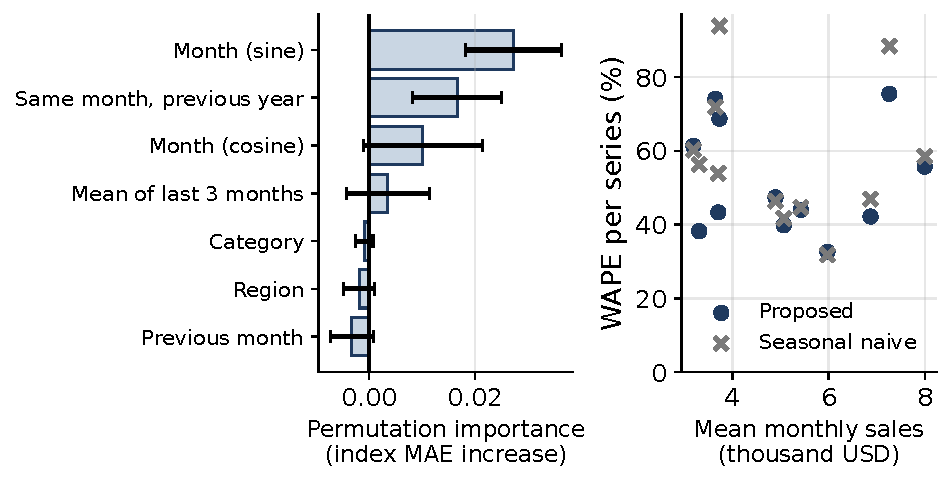
\includegraphics[width=\linewidth]{figures/importance_errors.pdf}
\caption{Izquierda: importancia por permutación de cada variable en el conjunto de prueba (aumento del MAE del índice al permutarla; media y desviación estándar de 30 repeticiones). Derecha: WAPE por serie del modelo propuesto y del ingenuo estacional frente a la venta mensual media de la serie.}
\label{fig:imp}
\end{figure}

\textbf{Errores por segmento.} El WAPE por serie va de 32.6\% (Muebles, Oeste) a 75.5\% (Tecnología, Este); tres de las cuatro series con mayor error son de Tecnología (68.7--75.5\%), consistente con su mayor concentración de atípicos. El modelo mejora al ingenuo estacional en 8 de las 12 series y en 7 de los 12 meses (Figura~\ref{fig:imp}, derecha).

\textbf{Errores por rango del objetivo.} Al dividir las observaciones en terciles de venta aparece una regresión a la media: en el tercil bajo (venta media de 1{,}558 USD) el modelo sobrestima en promedio 2{,}101 USD y su MAE (2{,}111 USD) es \emph{peor} que el del ingenuo estacional (1{,}819 USD); en el tercil alto (9{,}574 USD) subestima en 2{,}862 USD, aunque mejora al ingenuo (4{,}045 frente a 4{,}597 USD). Los residuos tienen media cercana a cero ($-35$ USD) y asimetría positiva (1.51): pocos errores grandes por subestimación (Figura~\ref{fig:pred}).

\textbf{Casos representativos.} Los cinco mayores errores son subestimaciones de picos: Tecnología en el Este en octubre (22{,}940 USD observados frente a 6{,}612 pronosticados) y noviembre, Tecnología en el Oeste en marzo, Oficina en el Centro en enero y Oficina en el Oeste en agosto. Son meses dominados por pocos pedidos de alto valor, imprevisibles con las variables disponibles. En el agregado, el modelo desplaza el pico de fin de año: subestima noviembre (118{,}448 USD observados frente a 87{,}831) y sobrestima diciembre (83{,}829 frente a 114{,}193), porque en 2017 el máximo ocurrió en noviembre, mientras que en 2016 había ocurrido en diciembre (Figura~\ref{fig:serie}).

\subsection{Discusión, limitaciones y amenazas a la validez}\label{subsec:discusion}

\textbf{Discusión.} Los resultados coinciden con la literatura en dos puntos y la matizan en uno. Primero, el sesgo de los modelos entrenados en dólares en un año de crecimiento es el esperado de métodos que no extrapolan, y la normalización por nivel lo corrige, como en los enfoques globales que escalan cada serie \cite{salinas2020,smyl2020}; el costo es un MAE por serie algo mayor, porque un pronóstico insesgado en presencia de asimetría positiva se aleja de la mediana que minimiza el error absoluto. SVR, cuya pérdida insensible a $\varepsilon$ es de tipo absoluto, muestra el mismo patrón por otra vía. Segundo, el modelo global no es peor que los modelos locales y es más estable al proyectar varios meses, en línea con \cite{monteromanso2021}. El matiz: la ventaja de los ensambles de árboles reportada en competencias con miles de series \cite{makridakis2022} no se observa aquí; con 288 observaciones, modelos de uno o dos hiperparámetros alcanzan errores estadísticamente equivalentes a una fracción del costo.

\textbf{Aplicación.} Reentrenado con 2015--2017, el modelo proyecta ventas de 913{,}423 USD para 2018, 24.6\% más que en 2017. A la luz de la prueba recursiva, esa cifra debe leerse con el margen medido en 2017: un desvío del total anual de $+3.4$\% y un WAPE mensual del total de 17.7\%, y sin garantía de que el crecimiento reciente se mantenga.

\textbf{Limitaciones y amenazas a la validez.} (i) \emph{Tamaño de muestra:} la prueba tiene 12 bloques mensuales; la potencia de las pruebas es baja y la aproximación asintótica de Diebold--Mariano y Giacomini--White ($n=11$) es frágil, de modo que la ausencia de significancia no demuestra equivalencia. (ii) \emph{Un solo conjunto de datos}, además de demostración: no se puede aplicar la prueba de Friedman ni afirmar generalización a otras empresas. (iii) \emph{Una sola partición temporal:} un esquema de origen móvil sobre varios años daría más bloques, pero la historia disponible no lo permite; el modelo tampoco se reentrena mes a mes durante 2017. (iv) \emph{Protocolo estadístico posterior:} las pruebas se definieron tras conocer las métricas agregadas de prueba; aunque se tomó la combinación estándar sin ajustarla al resultado, no es un registro previo estricto. (v) \emph{Dependencia:} promediar por mes absorbe la correlación entre series, pero la prueba bayesiana supone una estructura de correlación que aquí es solo aproximada. (vi) \emph{Variables:} no se usan promociones, precios ni calendario comercial, y el modelo solo produce pronósticos puntuales, sin intervalos. (vii) \emph{Fuga residual:} todas las variables usan únicamente meses anteriores y el preprocesamiento se ajusta dentro de cada pliegue; no se identificó fuga, aunque la elección de variables se benefició de un análisis exploratorio que incluyó 2017. (viii) \emph{Tiempos:} las mediciones dependen del equipo y varían entre ejecuciones, aunque no el orden de magnitud.

\section{Conclusiones}\label{sec:conclusiones}

El objetivo de superar simultáneamente a todos los modelos de referencia en error y en tiempo de cómputo no se cumplió, y así debe quedar dicho. El Random Forest global sobre el índice de ventas fue el modelo con menor error de validación cruzada y, en el año de prueba, mejoró al pronóstico ingenuo estacional, que representa la práctica actual, tanto en el error por serie como, sobre todo, en el total anual, donde pasó de una subestimación de casi 17\% a un desvío menor al 1\%. Pero esa mejora es un indicio y no una diferencia estadísticamente demostrada; frente a los otros siete regresores el modelo es indistinguible, uno de ellos tuvo un error por serie menor, y el Random Forest fue el más lento de ajustar y de ejecutar. El hallazgo más útil del estudio no es el ganador sino el intercambio que la ablación deja a la vista: trabajar con un índice libre de escala no reduce el error absoluto por serie, pero elimina el sesgo de nivel que afecta a los modelos entrenados en dólares y a SVR, y la codificación del mes es lo que mantiene estable la proyección a doce meses. Para planificar metas e inventario agregados, ese pronóstico sin sesgo es preferible a uno con menor error absoluto que subestima sistemáticamente.

Las limitaciones principales son un único conjunto de datos de demostración, doce meses de prueba que dejan poca potencia estadística, la ausencia de variables de promoción y precio, y pronósticos solo puntuales. Como trabajo futuro se propone: evaluar con origen móvil sobre conjuntos con más historia y sobre varios conjuntos de datos, para poder aplicar pruebas con potencia adecuada; simplificar el modelo retirando la historia reciente y comparar el Random Forest con un árbol único o un modelo lineal sobre el mismo índice, que aquí resultaron equivalentes y mucho más baratos; entrenar con pérdida cuantílica para producir intervalos y tratar de forma explícita la asimetría de las ventas; y reconciliar los pronósticos por serie con el total de la empresa.

\backmatter

\section*{Declaraciones}

\begin{itemize}
\item \textbf{Disponibilidad de datos:} Sample Superstore es un conjunto de datos público de demostración de Tableau Software \cite{superstore}. La copia utilizada (\texttt{data/raw/Sample - Superstore.csv}) y los datos procesados están en el repositorio del proyecto.
\item \textbf{Disponibilidad de código:} el código completo está en \url{https://github.com/AlexT09/SuperstorePython}. El ETL se ejecuta con \texttt{data/generate\_data.py}, el entrenamiento con \texttt{model/train\_model.py} y todas las tablas, pruebas estadísticas y figuras de este artículo con \texttt{paper/experimentos.py}; las versiones de las librerías están en \texttt{requirements.txt} y la semilla aleatoria es 42. El proyecto se presenta además como aplicación interactiva (\url{https://superstorepython.onrender.com}) y como libro (\url{https://alext09.github.io/SuperstorePython/}).
\item \textbf{Contribución de los autores:} ambos autores participaron en el diseño del estudio, la implementación, el análisis de resultados y la redacción, y aprobaron la versión final.
\item \textbf{Conflicto de intereses:} los autores declaran no tener conflictos de interés.
\end{itemize}

\bibliography{sn-bibliography}

\end{document}
